%%%%%%%%%%%%%%%%%%%%%%%%%%%%%%%%%%%%%%%%%
%Bert Text Abstractive Summarization
% LaTeX Template
% Version 1.4 (15/5/16)
%
% This template has been downloaded from:
% http://www.LaTeXTemplates.com
%
% Original author:
% Frits Wenneker (http://www.howtotex.com) with extensive modifications by
% Vel (vel@LaTeXTemplates.com) and Shane (shanepanter@boisestate.edu)
%
% License:
% CC BY-NC-SA 3.0 (http://creativecommons.org/licenses/by-nc-sa/3.0/)
%
%%%%%%%%%%%%%%%%%%%%%%%%%%%%%%%%%%%%%%%%%

%----------------------------------------------------------------------------------------
%	PACKAGES AND OTHER DOCUMENT CONFIGURATIONS
%----------------------------------------------------------------------------------------
\documentclass[twoside,twocolumn]{article}
\usepackage{biblatex}
\addbibresource{mybib.bib} % with extension

%\usepackage{blindtext} % Package to generate dummy text throughout this template 
\usepackage{listings}
\usepackage{xcolor}

\usepackage[sc]{mathpazo} % Use the Palatino font
\usepackage[T1]{fontenc} % Use 8-bit encoding that has 256 glyphs
\linespread{1.05} % Line spacing - Palatino needs more space between lines
\usepackage{microtype} % Slightly tweak font spacing for aesthetics

\usepackage[english]{babel} % Language hyphenation and typographical rules

\usepackage[hmarginratio=1:1,top=32mm,columnsep=20pt]{geometry} % Document margins
\usepackage[hang, small,labelfont=bf,up,textfont=it,up]{caption} % Custom captions under/above floats in tables or figures
\usepackage{booktabs} % Horizontal rules in tables

\usepackage{lettrine} % The lettrine is the first enlarged letter at the beginning of the text

\usepackage{enumitem} % Customized lists
\setlist[itemize]{noitemsep} % Make itemize lists more compact

\usepackage{abstract} % Allows abstract customization
\usepackage{graphicx}
\graphicspath{ {./images/} }
\renewcommand{\abstractnamefont}{\normalfont\bfseries} % Set the "Abstract" text to bold
\renewcommand{\abstracttextfont}{\normalfont\small\itshape} % Set the abstract itself to small italic text

\usepackage{titlesec} % Allows customization of titles
\renewcommand\thesection{\Roman{section}} % Roman numerals for the sections
\renewcommand\thesubsection{\roman{subsection}} % roman numerals for subsections
\titleformat{\section}[block]{\large\scshape\centering}{\thesection.}{1em}{} % Change the look of the section titles
\titleformat{\subsection}[block]{\large}{\thesubsection.}{1em}{} % Change the look of the section titles

\usepackage{fancyhdr} % Headers and footers
\pagestyle{fancy} % All pages have headers and footers
\fancyhead{} % Blank out the default header
\fancyfoot{} % Blank out the default footer
\fancyhead[C]{Bert-Text Abstractive Summarization $\bullet$ April 2021} % Custom header text
\fancyfoot[RO,LE]{\thepage} % Custom footer text

\usepackage{titling} % Customizing the title section

\usepackage{hyperref} % For hyperlinks in the PDF

\usepackage{biblatex}

\usepackage{graphicx}
\graphicspath{ {./images/} }

\usepackage{tablefootnote} % Add a table footnote

%Includes "References" in the table of contents
\usepackage[nottoc]{tocbibind}
%----------------------------------------------------------------------------------------
%	TITLE SECTION
%----------------------------------------------------------------------------------------

\setlength{\droptitle}{-4\baselineskip} % Move the title up

\pretitle{\begin{center}\Huge\bfseries} % Article title formatting
\posttitle{\end{center}} % Article title closing formatting
\title{Bert-Text Abstractive Summarization} % Article title
\author{%
\textsc{Josh Coward}\\[1ex] % Your name
\normalsize Boise State University \\ % Your institution
\normalsize \href{mailto:joshcoward@u.boisestate.edu}{joshcoward@u.boisestate.edu} % Your email address
\and % Uncomment if 2 authors are required, duplicate these 4 lines if more
\textsc{Ryan Pacheco}\\[1ex] % Second author's name
\normalsize Boise State University \\ % Second author's institution
\normalsize \href{mailto:ryanpacheco413@u.boisestate.edu}{ryanpacheco413@u.boisestate.edu} % Second author's email address
\and % Uncomment if 2 authors are required, duplicate these 4 lines if more
\textsc{Sajia Zafreen}\\[1ex] % Third author's name
\normalsize Boise State University \\ % Third author's institution
\normalsize \href{mailto:sajiazafreen@u.boisestate.edu}{sajiazafreen@u.boisestate.edu} % Third author's email address
}
\date{April 30, 2021} % Leave empty to omit a date
\renewcommand{\maketitlehookd}{%
\begin{abstract}
\noindent 
Text summarization is a process/technique to shorten an extended text such as books, news articles, blog posts, research papers, 
emails, and tweets in a coherent, fluent summary. It is one of the Natural Language Processing applications, which significantly 
impacts our lives with a spiking demand every day. With growing digital media and publishing, text summarization helps with deciding 
on whether an article/ document/ book is valuable or not. With the availability of textual data, it has become easier to train a model 
for text summarization. This paper discusses Text Abstractive Summarization using Bert to create a model that produces results comparable 
to Google's massive Pegasus model they developed and released back in June of 2020. We used the English language for our project as it's 
a language we can speak and understand. We also used the datasets to train our model consist of only English entries. We have used the 
CNN/Daily Main, SAMSum Corpus, and BillSum Corpus as our datasets.   
\end{abstract}
}

%----------------------------------------------------------------------------------------

\begin{document}

% Print the title
\maketitle


%----------------------------------------------------------------------------------------
%	ARTICLE CONTENTS
%----------------------------------------------------------------------------------------

\section{Introduction}
\lettrine[nindent=0em,lines=3]

Text Summarization summaries extended text while keeping coherent context. The increasing amount of unstructured data needs to be 
extracted in relevant summaries. There are different types of text summarization: Extractive and Abstractive. Extractive summarization 
generates a summary by selecting salient sentences or phrases from the source text, while abstractive methods paraphrase and restructure 
sentences to compose the summary. We focus on abstractive summarization in our work. There are many abstractive approaches based on a 
sequence-to-sequence model with a copy mechanism. However, some there are issues with these abstractive methods are: 1) because these 
methods use a left-context decoder while predicting each word, these methods do not have complete context. 2) as they do not use 
pre-trained contextualized language models on the decoder, the decoded does learn summary representation, context interactions, 
and language modeling together. 
BERT, which stands for Bidirectional Encoder Representations from Transformation, is designed to pre-train deep bidirectional representations 
from the unlabeled text by jointly conditioning both left and right context in all layers. As a result, the pre-trained BERT model can be 
fine-tuned with just one additional output layer to create state-of-the-art models for a wide range of tasks, such as question answering 
and language inference, without substantial task-specific architecture modifications.\par
BERT is conceptually simple and empirically powerful. It obtains new state-of-the-art results on eleven natural language processing tasks, 
including pushing the GLUE score to 80.5\% (7.7\% point absolute improvement), MultiNLI accuracy to 86.7\% (4.6\% absolute improvement), 
SQuAD v1.1 question answering Test F1 to 93.2 (1.5 points absolute improvement) and SQuAD v2.0 Test F1 to 83.1 (5.1 points absolute 
improvement).\footnote{See "Computation and Language", arXiv:1810.04805 }. \par
Bert has been very successful in textual entailment, name entity recognition, and machine reading comprehension. We have used the 
Bert-base-uncased pre-trained model for both the encoder and decoder, with the goal in mind of creating a model that resembles to Google's 
massive Pegasus model.

%------------------------------------------------

\section{Background}



%------------------------------------------------

\subsection{Works Cited}
We have used \cite{aksenov2020abstractive}, \cite{zhang2019pretraining} as reference. In the \cite{aksenov2020abstractive} paper, the 
text summarization model is based on the Transformer architecture. The architecture adopts the original model of Vaswami et al. (2017). 
On top of the decoder, they used a Pointer-Generator to increase the extractive capabilities of the network. In Paper \cite{zhang2019pretraining}, 
proposed 1. A natural language generation model based on BERT, making good use of the pre-trained language model in the encoder and decoder 
process, and the model can be trained end-to-end without handcrafted features. 2. A design a two-stage decoder process. In this architecture, 
our model can generate each word of the summary considering both sides’ context information. 3. To conduct experiments on the benchmark datasets 
CNN/Daily Mail and New York Times. Our model achieves a 33.33 average of ROUGE-1, ROUGE-2 and ROUGE-L on the CNN/Daily Mail, which is 
state-of-the-art. On the New York Times dataset, our model achieves about 5.6\% relative improvement over ROUGE-1. 
Our work doesn't differ much from the papers we referenced here \cite{aksenov2020abstractive}, \cite{zhang2019pretraining}. As BERT can't 
process sequences with more than 512 tokens, to deal with that our model is using overlapping subsection text of length 512 words and generating 
summaries for each of the individual subsections. In the end, a final summary across all those summaries. In the case of summaries, we didn't 
use a pre-trained summary model until the end.


%------------------------------------------------

\subsection{Datasets}

Our project used three datasets: \textbf{1) CNN/Dailymail, 2) SAMSum corpus, and 3) Billum corpus}. There are different datasets for text 
summarization. We tried to find datasets with "gold" summaries to compare our generated summaries with the "gold" summaries for our approach.\par 

The \textbf{CNN/Dailymail} is an English-language dataset containing just over 300k unique news articles written by journalists at CNN and 
the Daily Mail. We have used version 3.0.0, which can be used to train both abstractive and extractive summarization.\par
The data consists of news articles and highlight sentences. In the question answering setting of the data, the articles are used as the 
context and entities are hidden one at a time in the highlight sentences, producing Cloze style questions where the goal of the model is 
to correctly guess which entity in the context has been hidden in the highlight. In the summarization setting, the highlight sentences are 
concatenated to form a summary of the article. The CNN articles were written between April 2007 and April 2015. The Daily Mail articles were 
written between June 2010 and April 2015.
The model performance is measured by how high the output summary's ROUGE score for a given article is compared to the highlight written by 
the original article author. Zhong et al. (2020) report a ROUGE-1 score of 44.41 when testing a model trained for extractive summarization. 
See the Papers With Code leaderboard for more models.\footnote{See "Get To The Point: Summarization with Pointer-Generator Networks", 
https://www.aclweb.org/anthology/P17-1099}. There is a string for the article for each instance, a string for the highlights, and a 
string for the id.  The train set has 287,113, the validation set has 13,368, and the Test set has 11,490 instances in Split.

The \textbf{SAMSum} dataset contains about 16k messenger-like conversations with summaries. Conversations were created and written down 
by linguists fluent in English. The dataset reflects the proportion of topics of real-life messenger conversations.  It has 16369 
conversations distributed uniformly into 4 groups. Each instance contains an id string, a summary string, and a dialogue string.  
The train set has 14,732, the validation set has 818, and the test set has 819 instances in Split.  The summaries are annotated and 
assume they should 1) be short, 2) extract important pieces of information, 3)include names of interlocutors, and 4)be written in 
the third person. Each dialogue has only one reference of summary.\footnote{See "{SAMS}um Corpus: A Human-annotated Dialogue Dataset 
for Abstractive Summarization", https://www.aclweb.org/anthology/D19-5409} \par

The \textbf{BillSum} dataset summarizes the state bills of US Congressional and California states. It has several features: 1)text: 
bill text, 2) summary: summary of the bills, 3)title: title of the bills, 4)text\_len: number of chars in text, 5)sum\_len: number 
of chars in summary. The data field has a text string, a \cite{aksenov2020abstractive} summary string, and a title string. The train 
set has 18,949,  the ca\_test set has 1237, and the test set has 3269 instances in Split.\footnote{See "BillSum: A Corpus for Automatic 
Summarization of US Legislation", 1910.00523}



%------------------------------------------------

\section{Model and Approach}
One of the goals for our project was to ultimately create a custom natural language processing model capable of taking in text/articles of various lengths and outputting a condensed coherent summary of the original text. To do this we could have taken multiple approaches, we could have either done all of the text processing ourselves, build a custom tokenizer and language model in order to learn the meaning behind words and how they fit into the context around them and then use the resulting tokenizer and language model to train our text summerization model, this ultimately would take quite a long time to do and would require tons of computational power in which we do not have access to. The next best option which we went with was to use a pre-trained language model which has already been trained to learn the meaning of words and there surrounding context, the language model we went with was BERT. Having chosen BERT as our starting point for this project we needed to find a way to fine tune it on our given task at hand. 

The initial approach for this was to just follow the architecture from the Assignment A8 and just basically add an additional layer to a custom BERT class that consisted of our text data we planned on using, however we realized quite quickly that this approach wasn't going to work for the obvious reason of the type of data that was going to be outputted. No longer are we working with simple labels such as 0 and 1 for binary classification or 1,2,3,4... etc. for multi-class classification we actually needed to find a way to generate novel text, a task that what new to all of us. After conducting some brief research on how this task is commonly implemented we landed on the Encoder-Decoder model approach from article \cite{noauthor_leveraging_nodate}. The encoder-decoder model or sometimes referred to as seq2seq transformer models uses recurrent neural networks to make its predictions. They were developed originally for machine translation, where the ordinal language would be encoded and then it would be decoded into the language of choice. 

The approach for our task is quite similar, the encoder-decoder model would be trained on all of our data, the encoder will encode the article and then the decoder will decode the encoded article based on a set number of parameters such as length of outputted sequence and then output a summarized/condensed version of the encoded data. 

The first thing we have to do before we are able to actually train our model is preprocess the data by tokenizing both the articles and the handwritten summaries so that the text is converted to a computer readable format and so that the input and output text is mapped to the proper format so that the data can then be fed into the model for training without any errors. To do this we instantiated a Bert Tokenizer using the "bert-base-uncased" model and used its corresponding API to map the data to the right format. Now that the data is tokenized and mapped to the proper format we are able to instantiate a base encoder decoder model using Hugging Face's EncoderDecoderModel API. The base model consists of two separate language models, one to serve as the encoder and the other as the decoder. In our case we decided to use the "bert-base-uncased" model once again for both the encoder and decoder for simplicity sake (although using something like GPT-2 would have most likely yielded better results as it was designed as a decoder where Bert is designed with more general purpose uses in mind, so with that said it may be something to look into for future work). 

With our base model created we are finally able to start training our model on our preprocessed training and validation datasets. This however is where things started to not go as planned. Our goal with this custom model was to get results that were comparable to some of the current cutting edge models (perhaps this is naïvely overly ambitious) to do this of course we have to train on a ton of data. But with the nature of how Encoder Decoder algorithms work they are quite computationally heavy and it wasn't noticed until the time of writing this report that in fact these algorithms have been limited to only being used by large companies and institutions with large amounts of computational power for that very reason. So with that said, being that we all lacked huge NVIDIA specific GPUs that allowed us to optimize our code with CUDA. We were forced to train our models using only our CPUs and the small GPU that Google Collaborate would allow us to use. As a result we were only able to train on a relatively small subset of the data as the full model was estimated to take over 10,000 hours to train which obviously we do not have the time to do. This unfortunately resulted in really poor results when comparing both the rouge-1 and rouge-2 scores to current cutting edge models, not only that but the quality of the actual outputted summary was beyond terrible, it seemed to just output the most commonly found words in the article over and over again for the designated length of the outputted summary. 


%----------------------------------------------------------------------------------
\subsection{Pre Trained Model Comparison}

In order to gain a better understanding of BERT abstract text summarization, several pre-trained BERT summarizers to compare with one another and with our fine tuned BERT model. The models chosen were gathered from hugging face and are google/pegasus-cnn-dailymail, t5-base, sshleifer/distilbart-cnn-12-6, facebook/bart-large-cnn, nsi319/legal-led-base-16384, google/pegasus-newsroom, google/pegasus-wikihow, and ml6team/mt5-small-german-finetune-mlsum. These models were chosen by exploring the hugging face website and looking through the abstractive text summarization models while looking at which ones would provide interesting comparisions to our fine tuned BERT model. For example, two google pegasus models were chosen, google/pegasus-cnn-dailymail and google/pegasus-wikihow. Each of these models was trained on a different collection of text articles, providing a more complete view of the various pre-trained models, rather than just looking for ones trained on the same set of data.

In order to effectively compare these these classifiers they were first all initialized and loaded into a python dicitonary for access later, as shown below.

\begin{lstlisting}[language=Python]
summarizers = {}
for name in tqdm(sum_list):
    summarizers[name] = 
      pipeline(
        "summarization", 
        model=name,tokenizer=name)
\end{lstlisting}

Once the models were all loaded into the dictionary they were then all given the same 200 articles from the \textbf{1) CNN/Dailymail, 2) SAMSum corpus, and 3) Billum corpus} datasets. However the pre trained models have character limits on the text they will summarize. This causes errors when trying to just generate summaries for every single article in the datasets. In order to rectify this issue, a BERT extractive summarizer that can be installed via pip. The extractive summarizer shortens an article that is to long by removing all but what it views as the critical sentences. Once the article is shortened it can be through the pre trained models and have an abstractive summary generated. 



%------------------------------------------------

\section{Evaluation}

Once all the articles are summarized through by the 6 pre trained models the summaries are evaluated using two metrics. The first is rouge, which calculates the precision, recall, and fmeasure for each model when comparing the generated summaries to the "gold" summaries used for evaluation, precision, recall, and fmeasure are defined below. 

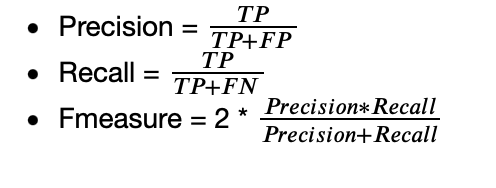
\includegraphics[width=0.45\textwidth,height=0.9\textheight,keepaspectratio]{report/metrics.png}

The second metric used was the SequenceMatcher simmilarity metric imported from the python difflib library. This library calculates a similarity score for two strings and returns a score as to how similar they are. When looking at the articles, we determined that a similarity score of 0.1 between the generated summary, and the "gold" summary shared the same main ideas. This similarity score was used to calculate a basic accuracy for each model, where if a generated summary had a similarity score > 0.1 it was considered "good". This was then used to compute an accuracy score where the number of good summaries is divided by the total number of generated summaries. The code below shows the model evaluations.

\begin{lstlisting}[language=Python]
sum_scores = {}
for model_name in tqdm(sum_preds):
    sum_scores[model_name] = {}
    good_score = 0
        pred = []
        gold = []
        for text_sum in range(
          len(sum_preds[model_name])):
            pred.append(sum_preds[model_name]
                [text_sum])
            gold.append(clean_sum[text_sum])
            score=similar(sum_preds[model_name]
                [text_sum], clean_sum[text_sum])
            if score > .1:
                good_score += 1
        try:
            good = rouge.compute(
                predictions=pred, 
                references=gold, 
                rouge_types=
                  ["rouge2"])["rouge2"].mid
        except:
            good = [0.0, 0.0, 0.0] 
        sum_scores[model_name]
          ['rouge'] = good
        sum_scores[model_name]
          ['similar']=
            good_score/len(summary)
\end{lstlisting}
This code takes into account the possibility that a model might not have generated any summaries for a given article. If this is the case then the precision, recall, and fmeasure are set to 0.0 as to not interfere with later comparisons. 

Once these metrics were calculated we were able to look at how each model did at summarizing the data. Unfortunatly due to the how long our fine tuned model was taking to train due to the limitations of our personal machines, and online GPU's no data was able to be collected to compare to the pre-trained models. However all six of the pre-trained models were able to be evaluated and compared. 

\begin{verbatim}
google/pegasus-cnn_dailymail:
	Precision: 0.004057214480304053
	Recall: 0.005905264789728774
	Fmeasure: 0.0045819246686427785
	Similar: 0.42
	
t5-base:
	Precision: 0.1073388727069371
	Recall: 0.14239013214035595
	Fmeasure: 0.1183132141131514
	Similar: 0.65
	
sshleifer/distilbart-cnn-12-6:
	Precision: 0.004520071790974368
	Recall: 0.0074084513715388985
	Fmeasure: 0.005479731712023811
	Similar: 0.415
	
facebook/bart-large-cnn:
	Precision: 0.005140301159330723
	Recall: 0.00741847862673695
	Fmeasure: 0.00584081807500133
	Similar: 0.42
	
nsi319/legal-led-base-16384:
	Precision: 0.047713374623433426
	Recall: 0.13309086083714433
	Fmeasure: 0.06875642452398892
	Similar: 0.51
	
google/pegasus-newsroom:
	Precision: 0.0032018573368585773
	Recall: 0.0057494030307497805
	Fmeasure: 0.003990393536896979
	Similar: 0.18
	
google/pegasus-wikihow:
	Precision: 0.008260233918128655
	Recall: 0.001940067674312532
	Fmeasure: 0.002754875848317157
	Similar: 0.175
	
ml6team/mt5-small-german-finetune-mlsum:
	Precision: 0.06754566523757385
	Recall: 0.060843013592276354
	Fmeasure: 0.05992201390563309
	Similar: 0.585
\end{verbatim}
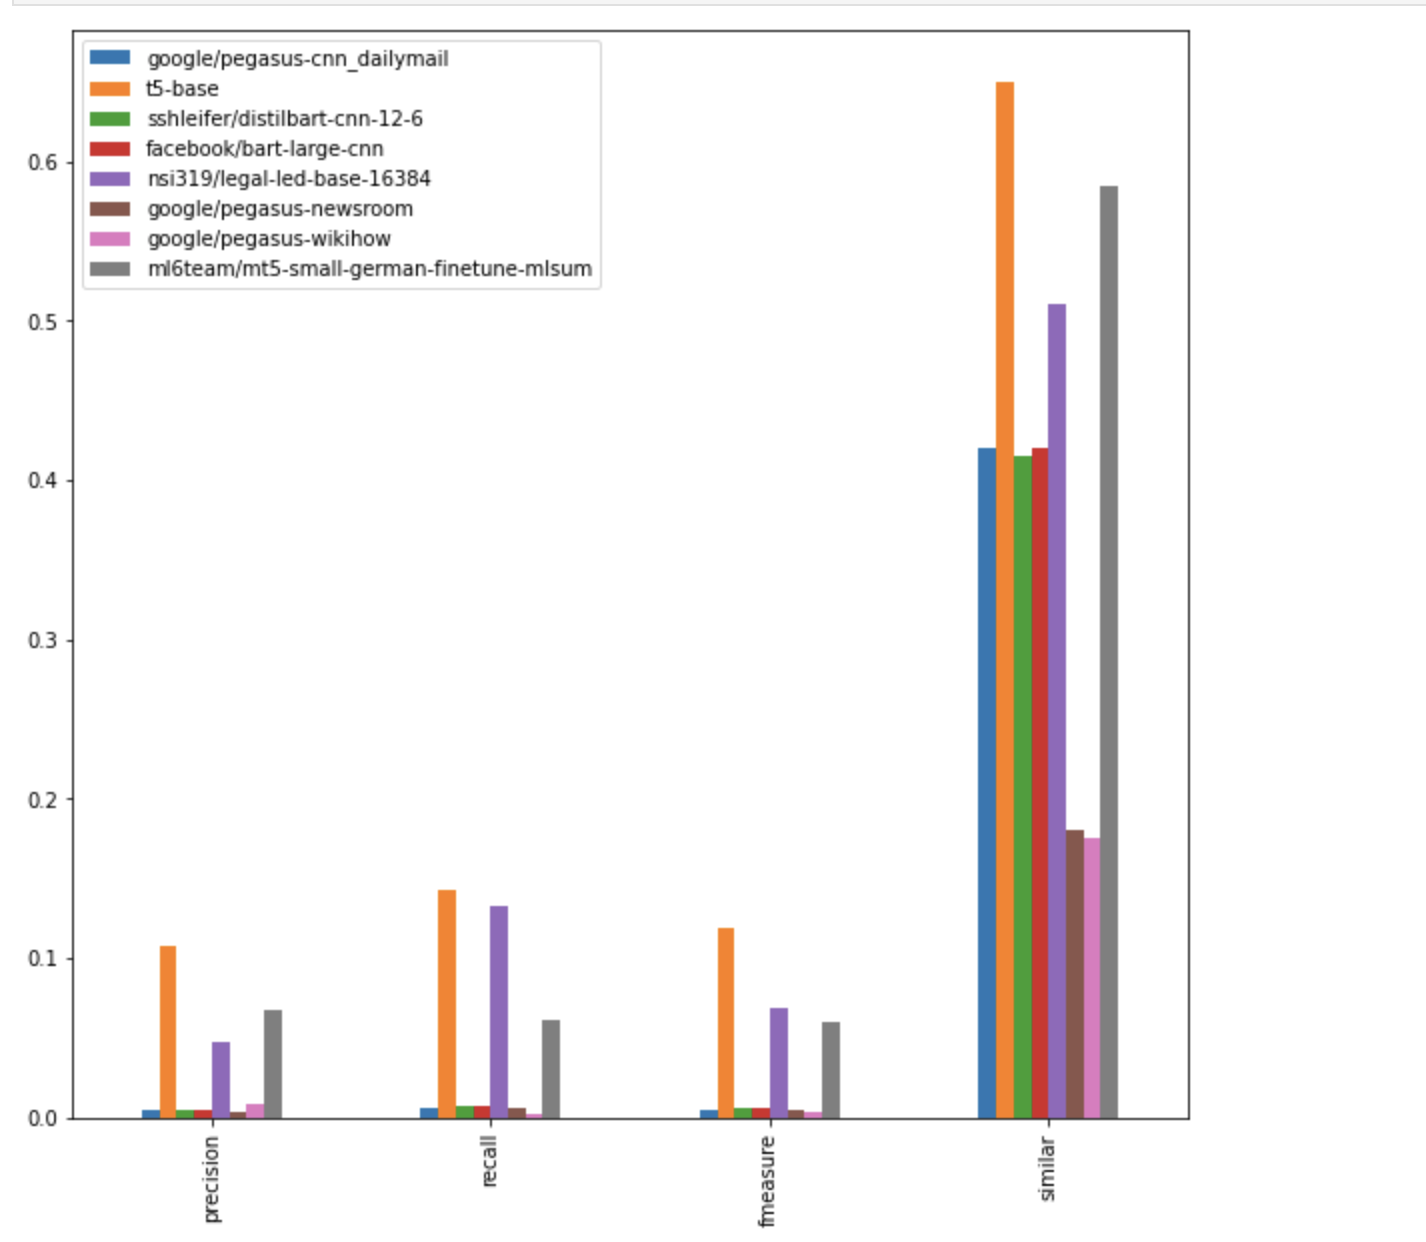
\includegraphics[width=0.58\textwidth,height=0.8\textheight,keepaspectratio]{report/cnn-graph.png}

Above shows how each pre-trained model did classifying the CNN/Dailymail dataset. As shown, t5-base, nsi319/legal-led-base-16384, and ml6team/mt5-small-german-finetune-mlsum had the best similarity metrics, and high metrics accross the board. Interestingly the pre-trained models trained on the CNN/Dailymail datasets such as google/pegasus-cnn-dailymail and facebook/bart-large-cnn struggled to have good metrics. Specifically their precision and recall were really low, signalling that these models generated a lot of false positives and false negatives. These metrics can be interpreted as more confusion being introduced due to the models being trained on the same data that is being used for evaluation.

The next dataset to be evaluated is the SAMSum corpus.
\begin{verbatim}
google/pegasus-cnn_dailymail:
	Precision: 0.06570140791970662
	Recall: 0.11194645893608307
	Fmeasure: 0.07676660531430701
	Similar: 0.965
	
t5-base:
	Precision: 0.0871608200405255
	Recall: 0.10878196145394188
	Fmeasure: 0.08892795374747745
	Similar: 0.95
	
sshleifer/distilbart-cnn-12-6:
	Precision: 0.08222619140159643
	Recall: 0.16857389607260176
	Fmeasure: 0.10307547627520189
	Similar: 0.965
	
facebook/bart-large-cnn:
	Precision: 0.1109204418673014
	Recall: 0.1506222918019447
	Fmeasure: 0.11705913865658535
	Similar: 0.97
	
nsi319/legal-led-base-16384:
	Precision: 0.048056536636149755
	Recall: 0.14721559364633643
	Fmeasure: 0.06862347378183611
	Similar: 0.93
	
google/pegasus-newsroom:
	Precision: 0.01969416070376323
	Recall: 0.04029707519377925
	Fmeasure: 0.02146641285892842
	Similar: 0.93
	
google/pegasus-wikihow:
	Precision: 0.05703333158776708
	Recall: 0.02338537494249275
	Fmeasure: 0.02896930473234471
	Similar: 0.895
	
ml6team/mt5-small-german-finetune-mlsum:
	Precision: 0.032227086778997535
	Recall: 0.05069437127612212
	Fmeasure: 0.03666129567374895
	Similar: 0.845
\end{verbatim}
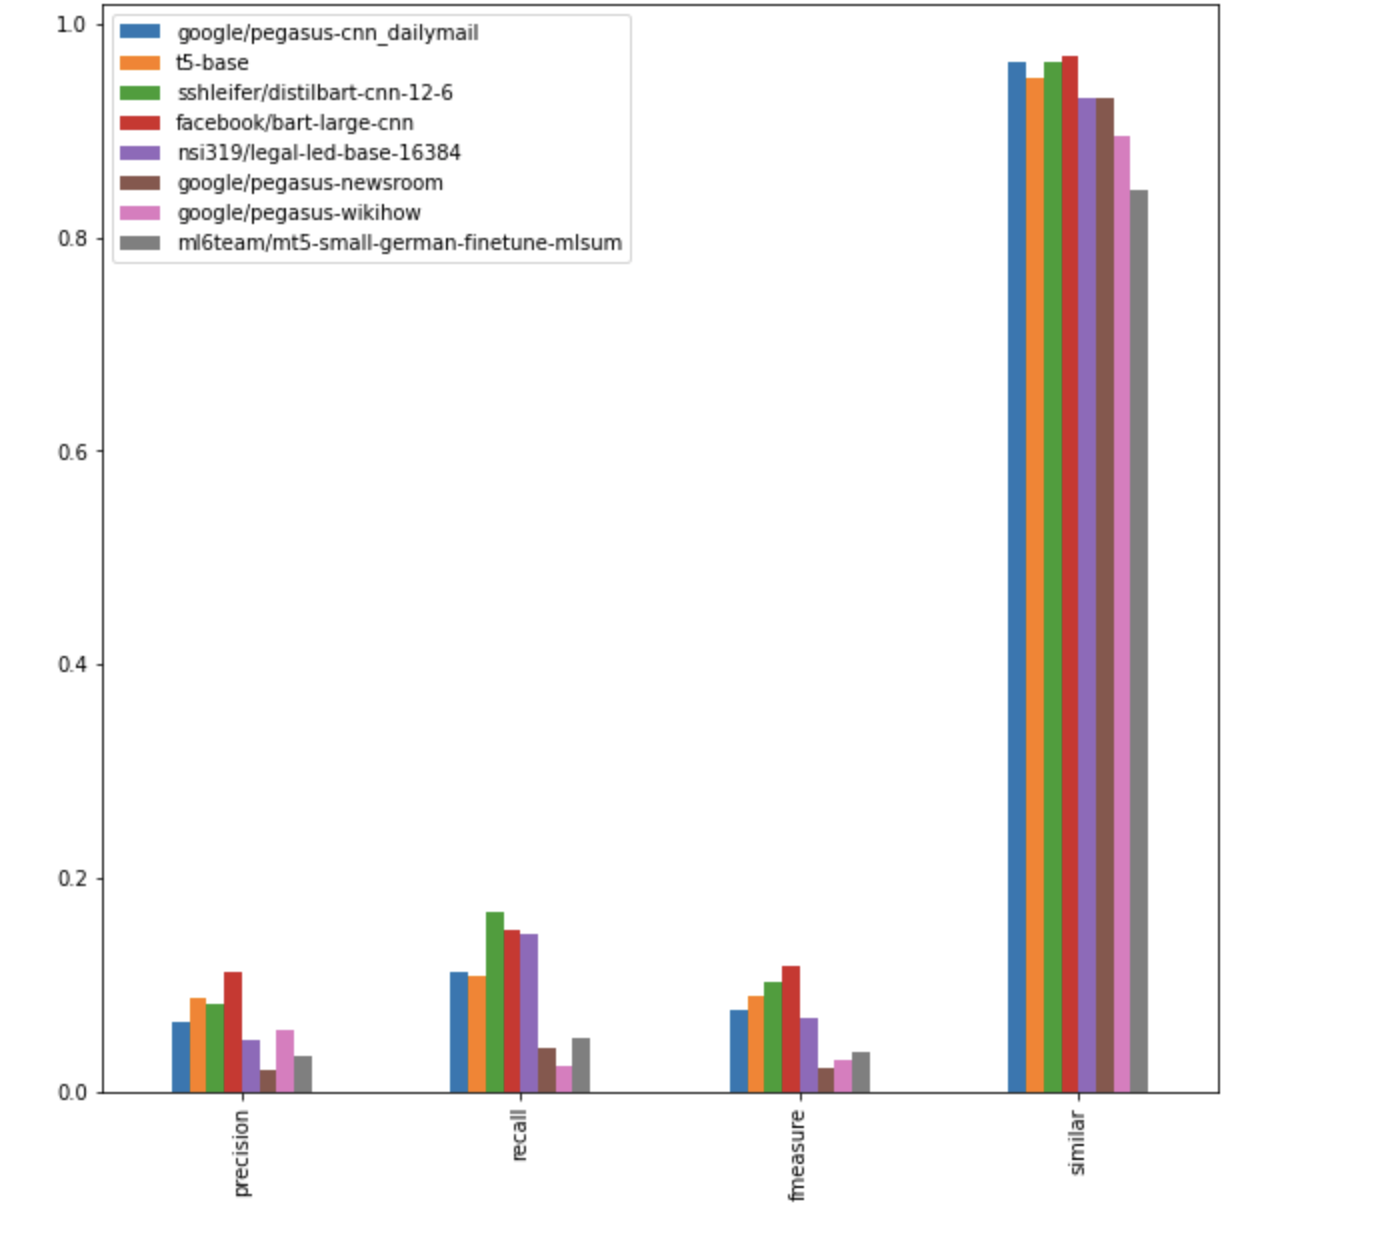
\includegraphics[width=0.58\textwidth,height=0.8\textheight,keepaspectratio]{report/graph-sam.png}

Here we see more parity between the models with facebook/bart-large-cnn and sshleifer/distilbart-cnn-12-6 preforming the best. Having the highest similarity scores, and the highest precision, recall, and fmeasure, two pre-trained models which were both trained using the CNN/Dailymail dataset interestingly preformed the best on a dataset seperate from what they were trained on.

The final dataset we looked at was the Billum corpus.
\begin{verbatim}
google/pegasus-cnn_dailymail:
	Precision: 0.034997246400968116
	Recall: 0.01585152779285387
	Fmeasure: 0.020187958372424764
	Similar: 0.005
	
t5-base:
	Precision: 0.2080614656568488
	Recall: 0.0842456195521589
	Fmeasure: 0.10906555198486713
	Similar: 0.18
	
sshleifer/distilbart-cnn-12-6:
	Precision: 0.0328451080507806
	Recall: 0.011291149429687435
	Fmeasure: 0.015812224174392167
	Similar: 0.005
	
facebook/bart-large-cnn:
	Precision: 0.030416521070095112
	Recall: 0.010306199164564775
	Fmeasure: 0.014132734541054626
	Similar: 0.005
	
nsi319/legal-led-base-16384:
	Precision: 0.11671223384360122
	Recall: 0.07259274110511799
	Fmeasure: 0.08094988869337535
	Similar: 0.075
	
google/pegasus-newsroom:
	Precision: 0.0
	Recall: 0.0
	Fmeasure: 0.0
	Similar: 0.0
	
google/pegasus-wikihow:
	Precision: 0.0
	Recall: 0.0
	Fmeasure: 0.0
	Similar: 0.0
	
ml6team/mt5-small-german-finetune-mlsum:
	Precision: 0.30615950365348016
	Recall: 0.05901749267334537
	Fmeasure: 0.08999198010632611
	Similar: 0.235
\end{verbatim}
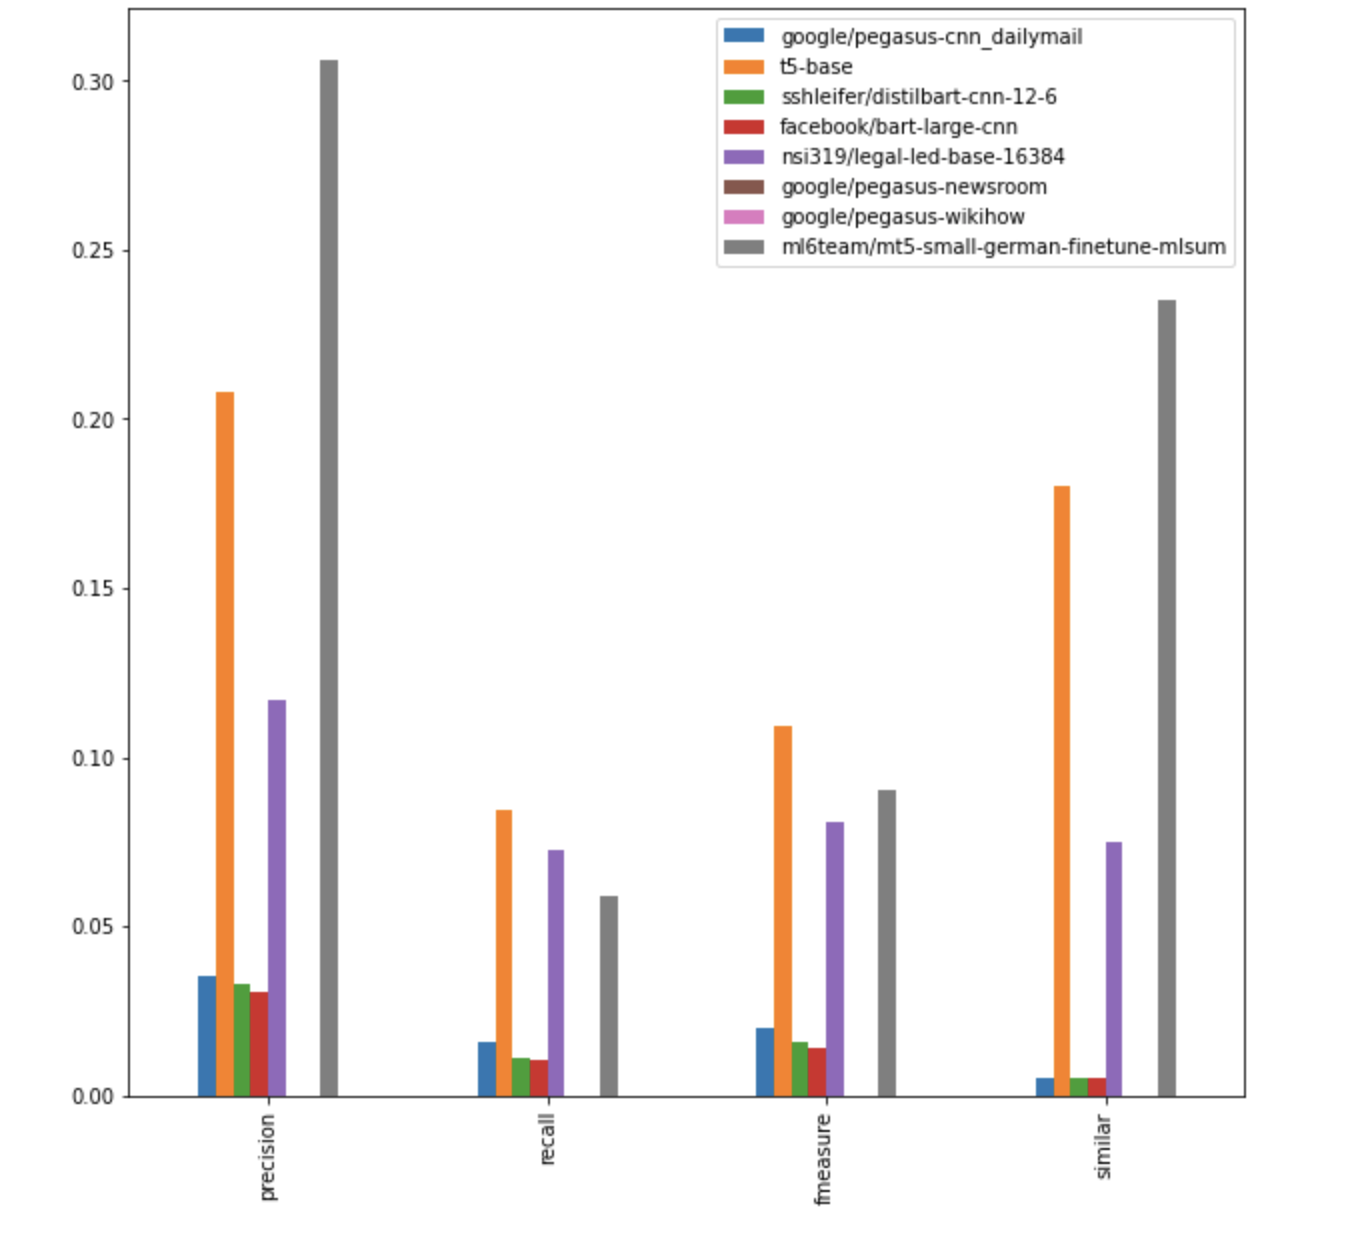
\includegraphics[width=0.58\textwidth,height=0.8\textheight,keepaspectratio]{report/graph-bill.png}

On this data we once again see the t5-base, nsi319/legal-led-base-16384, and ml6team/mt5-small-german-finetune-mlsum models out preforming the others. Once again having high similarity, precision, recall, and fmeasure scores. However two of the models, google/pegasus-newsroom and google/pegasus-wikihow, have scores of 0.0 across the board. This means that these models were not even able to generate summaries for this dataset.


%------------------------------------------------

\section{Implications}

When considering that for two out of the three data sets the same three models preformed the best. Leading to the interpretation that t5-base, nsi319/legal-led-base-16384, and ml6team/mt5-small-german-finetune-mlsum are more well suited for general text summarizaiton than the other models in this experiment. This is important to note in the future event that one wishes to preform abstract text summarization using pre-trained BERT models. Given the data collected one would be better to use t5-base, nsi319/legal-led-base-16384, or ml6team/mt5-small-german-finetune-mlsum rather than use google/pegasus-wikihow, google/pegasus-newsroom, google/pegasus-cnn-dailymail, facebook/bart-large-cnn, or sshleifer/distilbart-cnn-12-6.

%------------------------------------------------

\section{Conclusion}

%------------------------------------------------


%----------------------------------------------------------------------------------------
%	REFERENCE LIST
%----------------------------------------------------------------------------------------

%\section{References}    

%\cite{aksenov2020abstractive}

\printbibliography

  
%----------------------------------------------------------------------------------------

% FOR REFERENCE




\end{document}
